\section{Processes of the Central Dogma}
Up to this point, we have considered a variety of transport and biosynthetic
processes that are critical to acquiring and generating new cell mass. We now
turn our focus to some of the most important processes which \textit{must} be
undertaken irrespective of the growth conditions -- those of the central dogma.


\subsection{DNA Replication}
To successfully divide and produce viable progeny, the DNA must be
faithfully replicated and segregated into each nascent cell. Most bacteria
(including \textit{E. coli}) harbor a single, circular chromosome and can have
extra-chromosomal plasmids up to $\sim$ 100 kbp in length. We consider the
supply of the dNTP building blocks in Appendix Section "Additional Process of
the Central Dogma". Replication is initiated at a single region of the
chromosome termed the \textit{oriC} locus where a pair of replisomes, each
consisting of two DNA polymerase III, begin their high-fidelity replication of
the genome in opposite directions \citep{fijalkowska2012}. \textit{In vitro}
measurements have shown that DNA Polymerase III copies DNA at a rate of $\approx
600$ nucleotides per second (BNID: 104120). To replicate a single chromosome of
$\approx 5\times 10^6$ base pairs, two replisomes moving at their maximal rate
would copy the entire genome in $\approx$ 4000 s; well within out division time
of 5000 seconds.



% \begin{figure}
%   \centering{
%     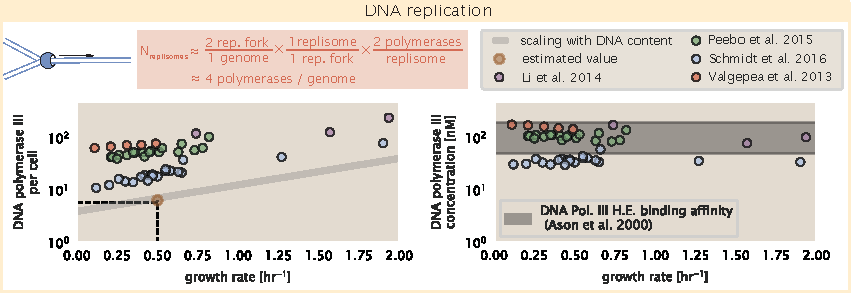
\includegraphics{main_figs/fig7_DNA_replication_main.pdf}
%     \caption{\textbf{Complex abundance estimates for dNTP synthesis and DNA
%     replication.} An estimate
%     for the minimum number of DNA polymerase holoenzyme complexes needed to
%     facilitate replication of a single genome. Points in the left-hand plot correspond
%     to the total number of DNA polymerase III holoenzyme complexes
%     ([DnaE]$_3$[DnaQ]$_3$[HolE]$_3$[DnaX]$_5$[HolB][HolA][DnaN]$_4$[HolC]$_4$[HolD]$_4$)
%     per cell. Right-hand plot shows the effective concentration of DNA polymerase III
%     holoenzyme (See Appendix Section "Estimation of Cell Size and Surface Area" for calculation of cell
%     size). Grey lines in left-hand panel show the estimated number of
%     complexes needed as a function of growth, the details of which are described
%     in the Appendix.} \label{fig:DNA_synthesis}
%      }
%     \figsupp[Estimate and observations of the abundance of ribonucleotide
%     reductase, a key component in dNTP synthesis.]{Estimate of the number of
%     ribonucleotide reductase enzymes needed to facilitate the synthesis of
%     $\approx 10^7$ dNTPs over the course of a 5000 second generation time. Points
%     in the plot correspond to the total number of ribonucleotide reductase I
%     ([NrdA]$_2$[NrdB]$_2$) and ribonucleotide reductase II ([NrdE]$_2$[NrdF]$_2$)
%     complexes. Grey lines in top panel show the estimated number of complexes
%     needed as a function of growth, the details of which are described in the
%     Appendix.}{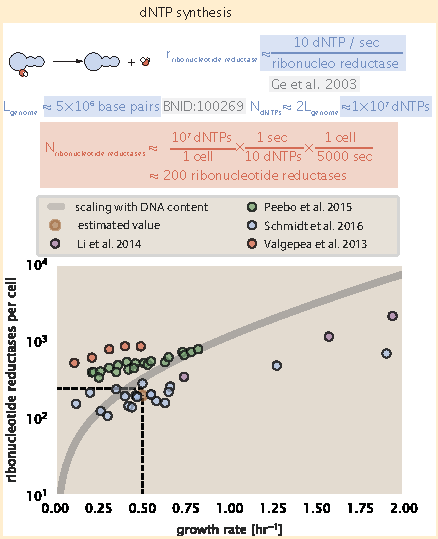
\includegraphics{main_figs/fig7-S1_dNTP_synthesis.pdf}}\label{figsupp:dntp}
% \end{figure}

\begin{figure}
    \centering{
    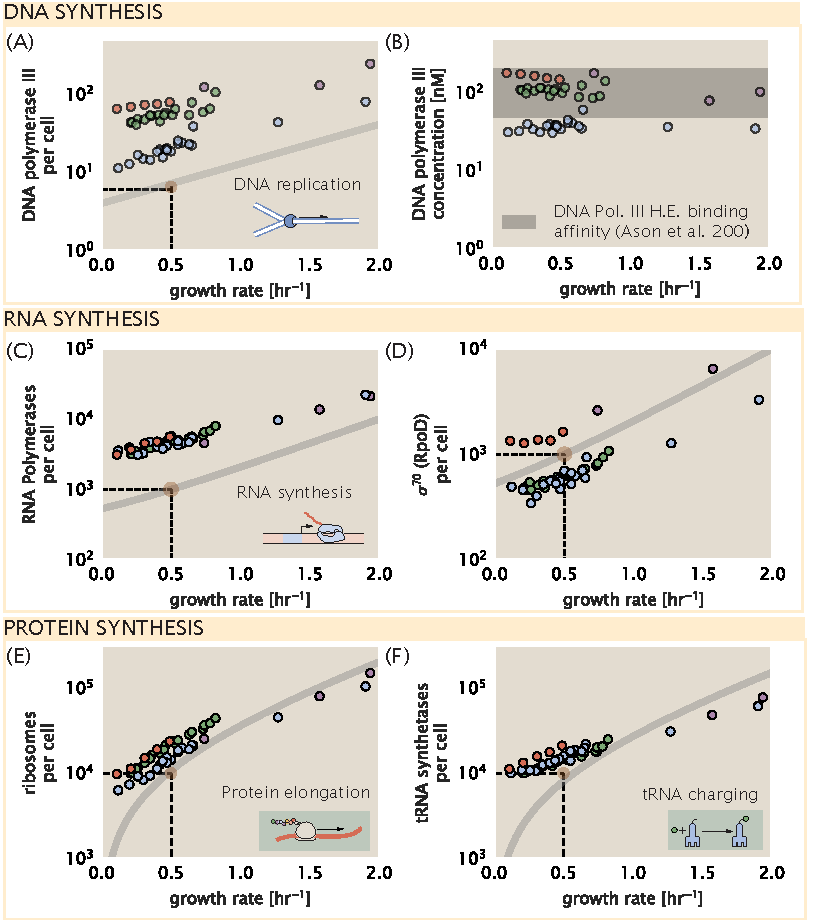
\includegraphics[width=0.6\textwidth]{main_figs/fig4_central_dogma.pdf}
    \caption{\textbf{Processes of the central dogma.}}
    \label{fig:central_dogma}
    }
\end{figure}

In rapidly growing cultures, bacteria like \textit{E. coli} can initiate as many
as 10 - 12 replication forks at a given time \citep{bremer2008, si2017},
suggesting  only $\approx 10$ are needed. However, as shown in
\FIG{central_dogma}(A), DNA polymerase III is nearly an order of magnitude more
abundant but still maintains the expected growth rate dependence. This
discrepancy can be  understood by considering its binding constant to DNA.
\textit{In vitro} characterization has quantified the $K_D$ of DNA polymerase
III holoenzyme to single-stranded and double-stranded DNA to be 50 and 200 nM,
respectively \citep{ason2000}. The concentration of DNA polymerase III across
all data sets apear in this range and cells vary theircopy number such that its
concentration is approximately equal to the dissociation constant to the DNA.
While the processes regulating the initiation of DNA replication are complex and
involve more than just the holoenzyme, these data indicate that the kinetics of
replication rather than the explicit copy number of the DNA polymerase III
holoenzyme is the more relevant feature of DNA replication to consider. In light
of this, DNA replication does not represent a rate-limiting step in
cell division. Interestingly, it is worth noting that for bacterium like \textit{C.
crescentus} whose chromosomal replication is initiated only once per cell cycle
\citep{jensen2001}, the time to double their chromosome indeed represents an
upper limit to their growth rate.
